\documentclass[conference]{IEEEtran}
\usepackage[utf8]{inputenc}
\usepackage[T1]{fontenc}
\usepackage{cite}
\usepackage{graphicx}
\usepackage{booktabs}
\usepackage{balance}
\usepackage{url}
\usepackage{hyperref}
\hypersetup{hidelinks}

\title{Design and Implementation of a Linux Resource Monitor Using Python, Concurrency, and SQLite Persistence}

\author{
\IEEEauthorblockN{Julio Cesar Blacio Machuca \qquad Ariel Jose Llumiquinga \~Nacato}
\IEEEauthorblockA{Carrera de Ingenier\'ia de Software\\
Universidad de las Fuerzas Armadas ESPE\\
Sangolqu\'i, Ecuador}
}

\begin{document}

\maketitle

\begin{abstract}
Monitoring system resources is essential to understanding the current state of an operating system, yet it can remain an abstract concept when examined only through isolated commands. This paper presents the design and implementation of a Linux terminal application developed in Python 3. The application organizes the six monitoring modules according to the Model--View--Controller pattern: CPU, memory and \textit{swap}, processes, connected users, filesystems, and networking. Data are obtained directly from the \texttt{/proc} virtual filesystem and, where appropriate, from native commands executed in a controlled manner. To meet operating-systems requirements, the application explicitly creates threads with \texttt{threading.Thread} and a child process with \texttt{os.fork()}, communicating through a pipe. Complete captures are persisted in SQLite and managed through CRUD operations. Verification performed on Ubuntu under WSL recorded 56 successful tests with no failures. The result is a traceable educational foundation that integrates observation, concurrency, and persistence without replacing system interfaces with high-level monitoring dependencies.
\end{abstract}

\begin{IEEEkeywords}
Linux, resource monitoring, Python, concurrency, SQLite, proc filesystem
\end{IEEEkeywords}

\section{Introduction}
Resource management makes it possible to relate the activity of processes, memory, storage, and communications to the observable behavior of an operating system. In particular, concepts such as processes, scheduling, memory, and input/output require concrete mechanisms that move from theoretical description to verifiable observation \cite{silberschatz2019}. Linux exposes part of that state through kernel interfaces and user-space commands, making it possible to build focused and transparent tools for educational purposes.

The \textit{Linux Resource Monitor} project addresses this need with an interactive console application intended to observe and record the state of a Linux computer without modifying processes, networking, memory, or filesystems. Its scope combines resource collection, an explicit demonstration of threads and processes, and persistence of complete captures. It is not intended to replace specialized tools or to serve as a performance benchmark.

This work contributes a single terminal application that brings together monitoring across six domains, direct \texttt{/proc} reading, native commands, explicit use of \texttt{threading.Thread} and \texttt{os.fork()}, and CRUD operations over SQLite. Its structure also provides automated evidence so that functional claims can be reviewed on Linux.

The technical objective is not limited to listing values: it preserves the provenance of each datum from its system source to presentation or storage. This required structured contracts among layers, a partial-failure policy for live queries, and a stricter persistence rule: a capture is stored only when it contains all six required modules. This distinction allows a changing system to be observed without confusing an incomplete live view with a complete historical record.

\section{Background and Related Work}
The \texttt{/proc} virtual filesystem publishes information generated by the kernel and running processes; it is therefore a suitable interface for querying counters and descriptors without requiring an intermediate database \cite{linuxproc}. This work uses it for CPU, memory, load, and network traffic, while sessions, processes, and mount points are obtained through native utilities that expose these system views.

The two source classes have different properties. Files under \texttt{/proc} represent state at the instant of each read, whereas utilities produce a snapshot whose composition may change before it is displayed. Consequently, the design does not require a process count to equal a later execution of \texttt{ps}; it requires well-formed records with traceable fields. Likewise, cumulative network counters are retained as bytes and packets and are not interpreted as rates without a measurement interval.

From an operating-systems perspective, separating collection, presentation, and coordination prevents terminal formatting from being mixed with resource access. This decision makes it easier to compare measurements, preserve them as captures, and manage errors by module. It also supports the study of the difference between threads that share a process and a child created with \texttt{fork()}, without concealing these mechanisms behind high-level monitoring libraries \cite{silberschatz2019}.

\section{Methodology}
\subsection{Incremental Development}
Development was organized over five weeks. The first defined requirements, the MVC architecture, and the relational schema; the second incorporated CPU, memory, and \texttt{/proc} reading; the third added disk, networking, users, and processes; the fourth integrated threads, \texttt{fork()}, and CRUD; and the fifth was dedicated to integration, tests, manuals, and evidence. This sequence kept each increment associated with a data source and observable acceptance criteria.

\subsection{Capture Flow}
A request for the overall state crosses four stages. First, the controller registers one collector function per module. Second, the coordinator creates one \texttt{Thread} object for each function, starts all six, and waits for completion. Third, it consolidates three separate structures: \texttt{datos}, \texttt{errores}, and \texttt{evidencias}; the last retains the module name, thread name, and UTC start and finish instants. Finally, the view can present available data and warn about errors. If the user chooses to record the state, the CRUD controller applies an additional validation before delegating the transaction to the repository.

The separation between querying and persistence is deliberate. During a live query, failure of one source does not discard information obtained by the others. By contrast, \texttt{consolidar\_captura} verifies that CPU, memory, disk, networking, processes, and users are present and that the error dictionary is empty. If a module is missing, a controlled error is raised and no write operation is opened for an incomplete capture.

\subsection{Sources and Calculations}
CPU information is described through \texttt{/proc/cpuinfo}, \texttt{/proc/loadavg}, and two readings of \texttt{/proc/stat}. Utilization is not inferred from load average; it is calculated from the deltas of total and idle time,
\begin{equation}
U_{CPU}=100\left(1-\frac{\Delta T_{idle}}{\Delta T_{total}}\right),
\end{equation}
where both counters come from the aggregate CPU line. For memory, the distinction between free and available memory is preserved: used memory is \texttt{MemTotal - MemAvailable}, while used \textit{swap} is \texttt{SwapTotal - SwapFree}. Networking uses \texttt{/proc/net/dev} for counters and \texttt{ip} for addresses; \texttt{ps}, \texttt{who}, and \texttt{df -P -B1} complement the process, user, and mounted-filesystem data.

\subsection{Data Contracts}
Models do not return terminal blocks. CPU and memory produce dictionaries; disk, networking, processes, and users produce lists of dictionaries, with one element per mount, interface, process, or session. Stable keys include \texttt{porcentaje\_uso}, \texttt{mem\_disponible\_mb}, \texttt{punto\_montaje}, \texttt{usuario\_propietario}, \texttt{direccion\_ip}, and \texttt{inicio\_sesion}. The controller preserves these structures, while the view adds units, rounds values to two decimal places, and builds ASCII tables.

Each parser accepts text and can therefore be tested without querying the current computer. Networking combines counters from \texttt{/proc/net/dev} with one address per interface: it prefers the first IPv4 address and uses IPv6 as a fallback; if no address exists, it retains \texttt{None}. Disk data are parsed as bytes from \texttt{df -P -B1} before conversion for display or persistence. For users, \texttt{inicio\_sesion} retains the instant reported by \texttt{who}; duration is calculated when displayed and does not replace the stored value.

\subsection{Concurrency and Safety}
Six independent threads, one for each module, are created before the application waits for their completion. Results, errors, and evidence are protected by a lock so that a partial response can be consolidated when a reading fails. The child process starts only after those threads have finished; this order avoids calling \texttt{fork()} while other threads are active. The child reads a load metric, communicates a JSON message through a pipe, and is reaped by the parent with \texttt{waitpid()}.

The demonstration also checks that no other threads are active before creating the child. Parent and child close the pipe end they do not use; the child terminates with \texttt{os.\_exit()}, and the parent converts the state returned by \texttt{waitpid()} into an exit code. A nonzero code or an empty pipe becomes a comprehensible error. The database does not participate in this flow, and no SQLite connection is shared with worker threads or with the child process.

\subsection{Failures and Changing State}
Commands are executed with an argument list, captured standard output and error, text mode, a five-second timeout, \texttt{LC\_ALL=C}, and no \texttt{shell=True} \cite{pythonsubprocess}. A nonzero return becomes a \texttt{RuntimeError}; a missing command, timeout, unavailable \texttt{/proc} file, or incomplete content propagates an exception that the worker records under the module name. Thus, the menu receives controlled messages instead of an abrupt termination.

Parsers ignore empty or nonconforming lines when they can continue and reject missing mandatory fields when the result would lose meaning. This criterion matters for tables that change during observation: a process may terminate between two queries, and an interface may have no IP address. The application accepts empty lists and unavailable addresses but does not invent values to complete a capture.

\subsection{Verification Strategy}
Unit tests validate parsing functions against sample files so that their results do not depend solely on the current machine. Persistence tests use temporary SQLite databases and cover CRUD operations and cascade deletion. Integrations requiring \texttt{fork()} are explicitly limited to Linux. The documented execution was performed on Ubuntu under WSL; therefore, this article does not extend that evidence to other systems.

Verification also covers contracts between layers: the controller preserves partial errors, an incomplete capture is rejected, connections enable foreign keys, update affects only metadata, and deletion removes child rows. Interface tests exercise invalid options, nonpositive identifiers, deletion cancellation, \texttt{EXITO}, \texttt{ADVERTENCIA}, and \texttt{ERROR} messages, and limits for long listings.

\section{Solution Architecture and Development}
\subsection{MVC Separation}
Fig.~\ref{fig:arquitectura} summarizes the organization. The model reads and transforms system data and encapsulates the SQLite repository. The view requests keyboard input and presents menus, tables, and messages. The controller coordinates collection, validation, concurrency, and the CRUD flow. This separation preserves structured data contracts among layers and prevents SQL queries or \texttt{/proc} reads in the view.

The \texttt{MonitorController} facade supports requesting either one module or the overall state without exposing how collection occurs. \texttt{CrudController} receives the concurrent result, requires a complete capture, and translates SQLite failures into an application exception. The repository is the only component that knows SQL statements; consequently, terminal navigation and integrity rules can be tested with doubles without executing Linux commands.

\begin{figure}[t]
\centering
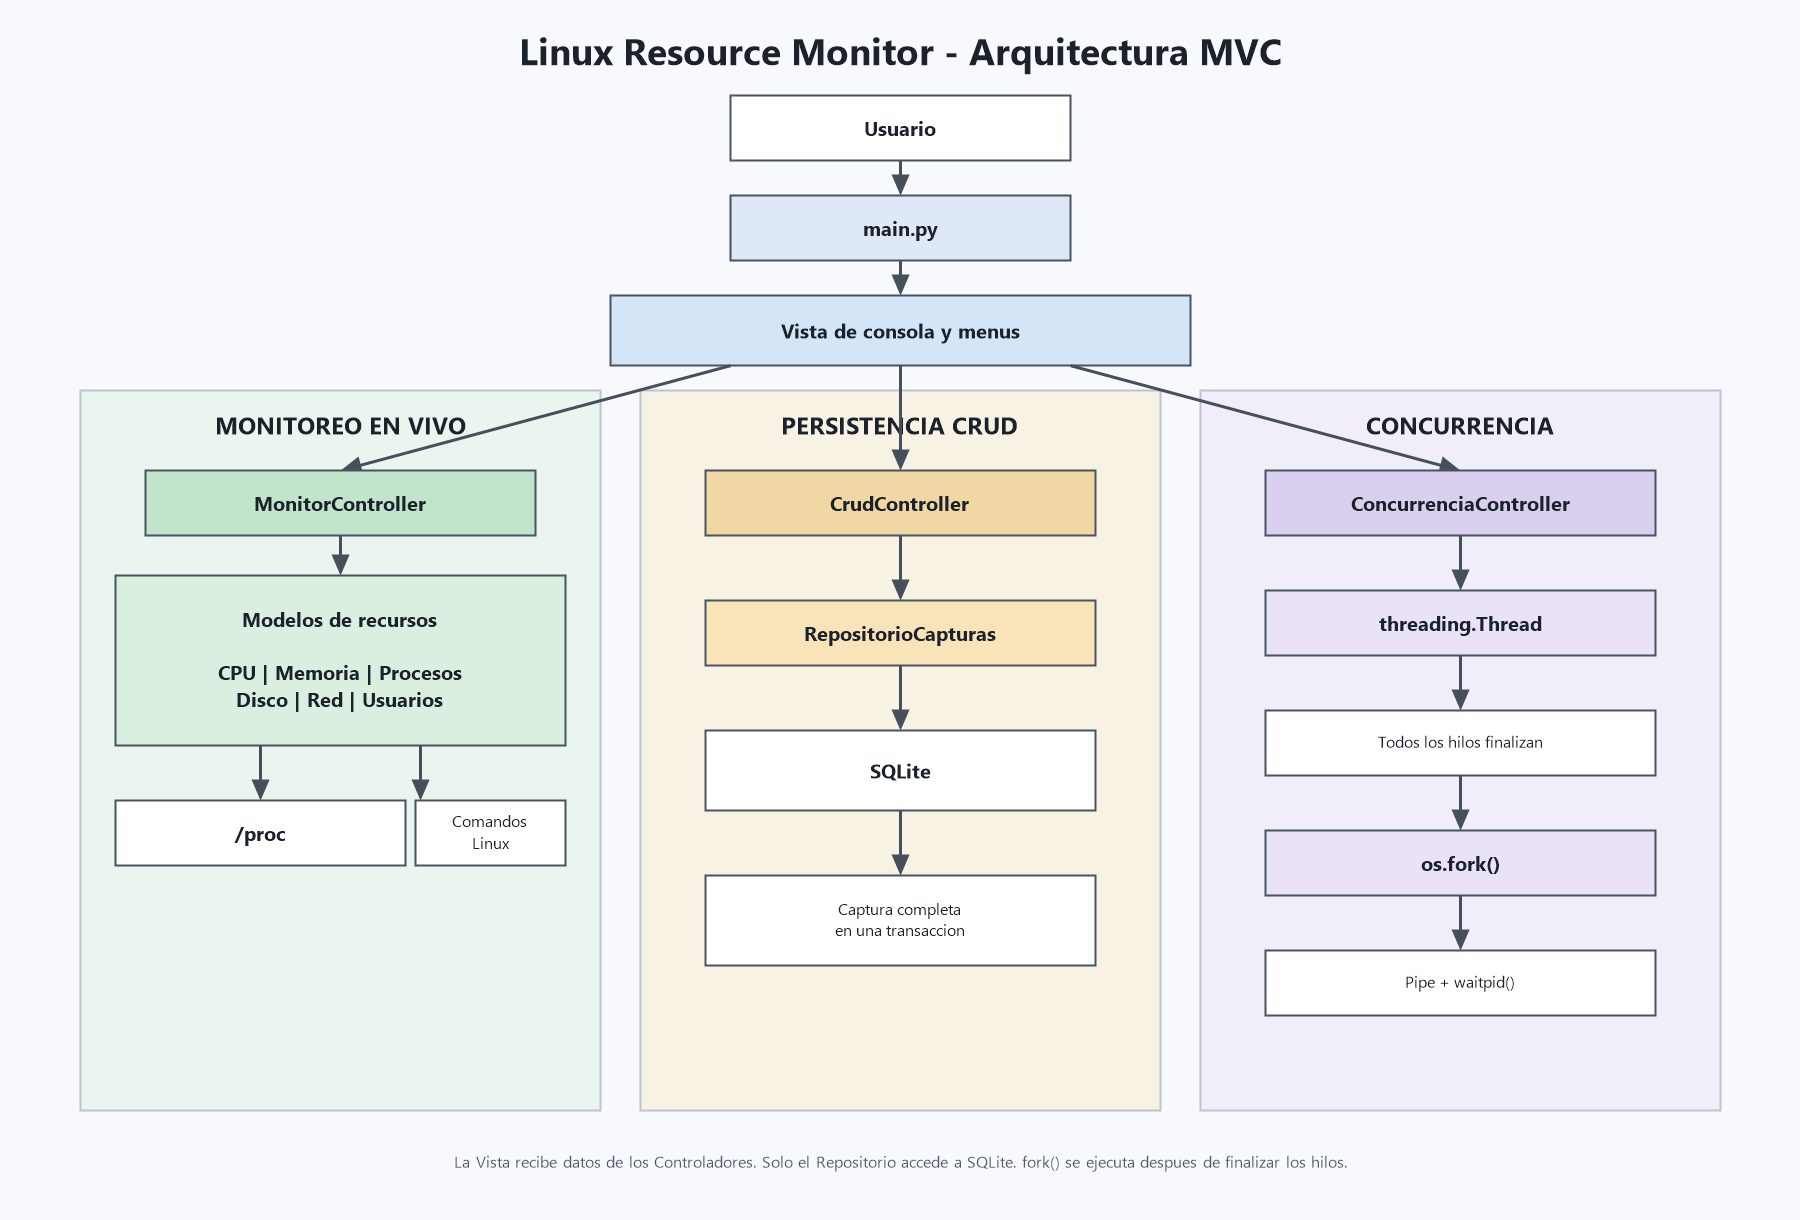
\includegraphics[width=\columnwidth]{figuras/arquitectura_actual.png}
\caption{MVC architecture, concurrent collection, and monitor persistence.}
\label{fig:arquitectura}
\end{figure}

\subsection{Monitoring Modules}
Table~\ref{tab:fuentes} relates each module to its primary source and the result delivered to the controller. Command invocations use argument lists, captured output, timeouts, and no \texttt{shell=True}; using \texttt{subprocess} preserves a clear boundary between the application and system commands \cite{pythonsubprocess}. The Python interfaces used for processes and threads correspond to the documented \texttt{os} and \texttt{threading} APIs \cite{pythonos,pythonthreading}.

\begin{table}[t]
\caption{Traceability between module, source, and collected data.}
\label{tab:fuentes}
\centering
\footnotesize
\begin{tabular}{@{}p{0.16\columnwidth}p{0.30\columnwidth}p{0.44\columnwidth}@{}}
\toprule
Module & Primary source & Collected data \\
\midrule
CPU & \texttt{/proc/cpuinfo}, \texttt{/proc/stat}, \texttt{/proc/loadavg} & Logical processors, model, frequency, load, and utilization \\
Memory & \texttt{/proc/meminfo} & Total, free, available, used, and \textit{swap} \\
Processes & \texttt{ps} & PID, name, state, and owner \\
Users & \texttt{who} & Username, terminal, and login start time \\
Disk & \texttt{df -P -B1} & Mount point, bytes, and utilization percentage \\
Network & \texttt{/proc/net/dev}, \texttt{ip} & Interface, address, and traffic counters \\
\bottomrule
\end{tabular}
\end{table}

The CPU module separates load from utilization: the three load values come from \texttt{/proc/loadavg}, whereas the percentage uses deltas from \texttt{/proc/stat}. The count is named logical processors because it comes from \texttt{processor} entries in \texttt{/proc/cpuinfo}; it is not presented as physical cores. Memory parsing validates five mandatory fields before converting KiB to MiB. Processes, users, and disk each parse one invocation of \texttt{ps}, \texttt{who}, or \texttt{df}, respectively, preserving a snapshot consistent with the invoked source.

\subsection{Concurrency and Persistence}
Collection starts the six \texttt{Thread} objects, joins them before consolidating the result, and retains errors by module. The child process is created through \texttt{os.fork()}, sends its data through a \texttt{pipe}, and is reaped without leaving orphan processes. This sequence makes the difference between thread coordination and interprocess communication explicit.

Captures are stored in a main table with related CPU, memory, disk, process, network, and user metrics. Each connection enables foreign keys, and every complete capture is written in one transaction, so a required failure rolls back the operation. The relationships use cascade deletion to remove associated metrics when a capture is deleted \cite{sqlitefk,sqlitetransactions}. CRUD supports creating, listing, and consulting captures, updating their metadata, and deleting them through the repository.

The relational design distinguishes cardinalities. CPU and memory have a one-to-one relationship with \texttt{capturas}: their primary key is also a foreign key. Disk, processes, networking, and users have one-to-many relationships and their own keys because a capture may include several elements of each type. The parent table retains date, label, comment, and recording user; update changes only the label and comment, never observed metrics.

Writing opens an independent connection and enters the transaction context before inserting the parent row and the six metric families. If a required key is absent, a contract type is invalid, or SQLite rejects a row, the context rolls back the set and the \texttt{finally} block closes the connection. During reading, the repository reconstructs the same contract used by the view: one dictionary for CPU and memory and lists for the one-to-many relationships.

\subsection{Terminal Interface Criteria}
The main and history menus use numbered options. Invalid input keeps the loop active; identifiers must be positive integers, and deletion requires the user to type \texttt{SI}. Process and filesystem listings are initially limited to 20 rows and state how many records are displayed relative to the total. These decisions prevent a large snapshot from displacing terminal context indefinitely.

Output does not depend on color. Percentages are accompanied by \texttt{NORMAL}, \texttt{ADVERTENCIA}, or \texttt{CRITICO}; values include units and two decimal places, and the overall state includes an update timestamp. Missing values are expressed as \emph{No disponible} or with specific empty-list messages. The interface therefore remains understandable in a plain-text terminal and through keyboard operation.

\section{Results and Validation}
Table~\ref{tab:resultados} summarizes an execution verified on July 12, 2026, on Ubuntu under WSL. The suite was run with \texttt{python3 -m unittest discover -s tests}; the other records exercised the monitoring controller, a temporary SQLite repository, and the concurrency demonstration. The values are a functional verification snapshot, not a performance benchmark or a platform comparison.

\begin{table}[t]
\caption{Verified results from the documented execution.}
\label{tab:resultados}
\centering
\footnotesize
\begin{tabular}{@{}p{0.25\columnwidth}p{0.43\columnwidth}p{0.20\columnwidth}@{}}
\toprule
Validation & Result & Status \\
\midrule
Full suite & 56 tests & 0 failures \\
Overall state & 6 modules & 0 errors \\
SQLite CRUD & Create/list/update/delete & Correct \\
Concurrency & 6 threads + 1 child & Exit status 0 \\
\bottomrule
\end{tabular}
\end{table}

The overall-state evidence recorded the CPU, memory, disk, process, network, and user modules with an empty error dictionary. In the persistence test, a capture was created, listed, had its metadata updated, and was deleted; the final listing contained no records. In the concurrency demonstration, six pieces of evidence with \texttt{monitor-} names and start and end markers were produced, followed by a child with a PID different from the parent's and an exit code of zero.

The suite combines deterministic tests and integration checks. Parsers for CPU, memory, disk, networking, processes, and users consume fixture files; the repository is created in a temporary directory and verifies both the reconstructed detail and cascade behavior; controllers are exercised with replaceable collectors and repositories; and Linux cases validate the integrated flow and a real \texttt{fork()}. This composition reduces dependence on ephemeral values without removing the final check on the target system.

Acceptance criteria were interpreted according to the nature of each datum. Key sets and formulas are required for CPU and memory, command records must be parseable, networking retains one primary address or explicit absence, the live view continues after partial failures, and history writes remain atomic. Exact equality is not required between counts taken at different instants, and observed execution times are not generalized.

\begin{figure}[t]
\centering
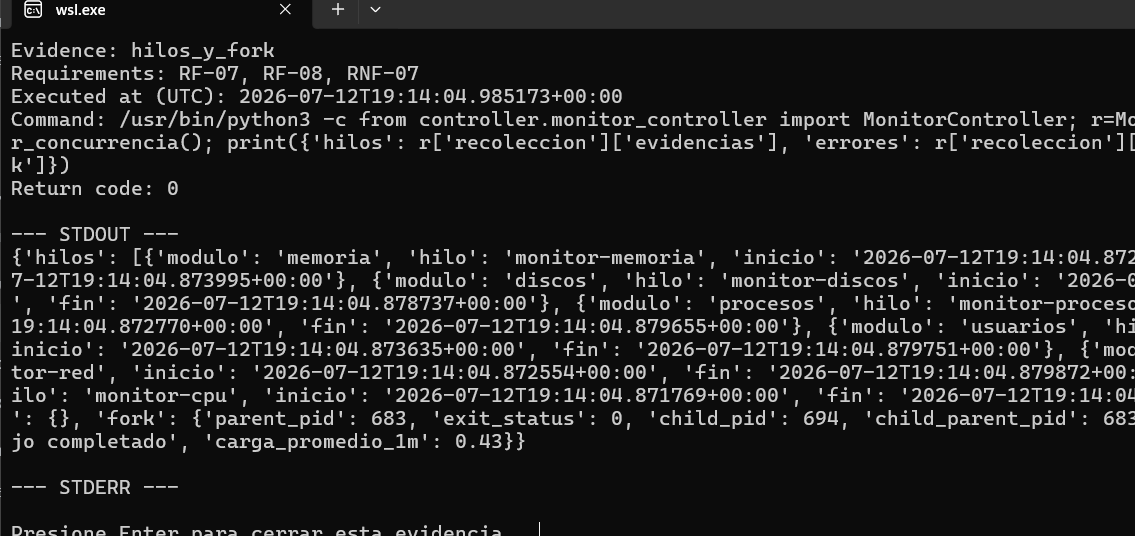
\includegraphics[width=\columnwidth]{figuras/evidencia_hilos_fork.png}
\caption{Evidence of six threads and one child process running under WSL.}
\label{fig:concurrencia}
\end{figure}

\balance
\section{Conclusions}
The monitor integrates the functional requirements for observing CPU, memory, processes, users, disk, and networking in a Linux terminal application. MVC separation keeps resource reading, coordination, and presentation distinct; in turn, the repository centralizes SQLite persistence and CRUD operations.

The demonstration of six threads and one child illustrates a relevant ordering decision: threads finish before \texttt{fork()} begins, and the parent retrieves the child through a pipe and \texttt{waitpid()}. The transaction for every complete capture and cascading foreign keys support the consistency of stored data. The documented verification supports the behavior described without attributing performance properties to it.

As limitations, the readings depend on the available Linux interfaces and represent changing system states. Future work may study portability in the collection layer or longer-duration samples while preserving the architectural separation and without claiming that these extensions form part of the current version.

\bibliographystyle{IEEEtran}
\bibliography{referencias}

\end{document}
